\documentclass[conference]{IEEEtran}
% *** GRAPHICS RELATED PACKAGES ***
%
%\ifCLASSINFOpdf

%\else

%\fi

\usepackage{amssymb}
\usepackage{multirow}
\usepackage{rotating}
\usepackage{amsmath}
\usepackage{float}
\usepackage{gensymb}

\usepackage[labelfont=scriptsize]{caption}
\renewcommand{\thefigure}{\arabic{figure}}
\renewcommand{\thetable}{\arabic{table}}

%\usepackage[table,xcdraw]{xcolor}
%\usepackage{graphicx}
\usepackage[utf8]{inputenc}
%\usepackage[english]{babel}
\usepackage[backend=biber,style=ieee,sorting=ynt]{biblatex}
\addbibresource{reference.bib}

\begin{document}

\title{Applied Machine Learning Project 3 \\ Digits Classification (Team: RND)}

\author{\IEEEauthorblockN{Liu Liu}
\IEEEauthorblockA{McGill University\\
liu.liu2@mail.mcgill.ca}
\and
\IEEEauthorblockN{Nissan Pow}
\IEEEauthorblockA{McGill University\\
nissan.pow@mail.mcgill.ca}
\and
\IEEEauthorblockN{Robert Wenger}
\IEEEauthorblockA{McGill University\\
robert.wenger@mail.mcgill.ca}}

% make the title area
\maketitle

% As a general rule, do not put math, special symbols or citations
% in the abstract
\begin{abstract}
In this machine learning paper, we analyzed images of hand-written digits (from 0 to 9), and classified them using several different machine learning algorithms. We used and compared Logistic Regression, feed-forward Neural Network (NN) trained by backpropagation, linear Support Vector Machine (SVM), and convolutional Neural Network (cNN). We obtained a score of 0.9304 on the public test set on the Kaggle website using the convolutional Neural Network method. We will present the details of the image analysis, and the testing and validation results for the different algorithms in this paper. In addition, we will also discuss the significances of our approach and methodology.
\end{abstract}

\IEEEpeerreviewmaketitle

\section{Introduction}
The classification of images with hand-written digits is a common and interesting problem in Machine Learning (ML). In everyday life, machines are often faced with this problem without any human input. For example, a bank machine can efficiently and accurately classify the hand-written digits on a cheque with higher accuracy than a human observer \cite{lecun-98, Schmidhuber:2012:MDN:2354409.2354694}. Given that the handwriting of every individual is unique, this results in large number of variations for each digit, making the classification of hand-written digits a difficult machine learning problem.

Another layer of complexity for using machine learning algorithms to classify digits is that there are 10 classes representing the digits from 0 to 9. Multi-class classification is a commonly faced problem, and the machine learning algorithms often need to be adapted to create decision boundaries for multiple classes \cite{bishop2006pattern}. In addition to designing an algorithm that is robust to the variation of individual handwriting, we seek algorithms that are robust to lighting, rotation of the digits, and the background overlaid on the images.

In this paper, the dataset is based on the well used MNIST dataset (LeCun, Cortes, Burges: http://yan.lecun.com/exdb/mnist/). In addition, the images were modified as described below to increase the difficulty of the task. We fully implemented the logistic regression method and a feedforward Neural Network (NN) trained by backpropagation to classify the images. In addition, we used a linear Support Vector Machine (SVM) from Matlab and scikit-learn toolboxes \cite{scikit-learn}. We also used a convolutional Neural Network (cNN) from Matlab \cite{IMM2012-06284} and Python toolboxes \cite{jia2014caffe}. We found that the cNN outperformed the other methods on average by around 0.5000 in classification accuracy. We will present the details of the analysis and the results, and then discuss the significances of our approach and methodology.

\section{Data Pre-processing Methods}
The dataset is based on the well used MNIST dataset (LeCun, Cortes, Burges: http://yan.lecun.com/exdb/mnist/). In addition, the digit images were modified using the following transformations to increase the difficulty of the task:
\begin{itemize}
\item Embossing of the digit with fixed lighting position that is not given.
\item Rotation by a random angle from [0,360] \degree.
\item Rescaling from $28 \times 28$ pixels to $48 \times 48$ pixels.
\item A random patch from a random texture pattern of the Brodatz dataset \cite{vn526306} was overlaid on the background. The MNIST digits were thresholded at 0.1 where for every pixel, the pixel from the MNIST digit was used if its intensity is higher than 0.1 or else the pixel from the texture was used.
\end{itemize}
The dataset was constructed by researchers from the LISA lab at the University of Montreal (Pierre Luc Carrier and Aaron Courville). The script used to construct the dataset can be found here (make\_mnistplus.py)\\
{\scriptsize https://github.com/lisa-lab/pylearn2/blob/master/pylearn2/scripts/datasets}.

To undo these transformations, we attempted to both remove the random texture background and to unrotate the digits. To remove the random texture background, we decided to look at ways that can help segment the numbers from the texture backgrounds, which could then simplify the classification problem by having an easier image to look at. We did this by using the ilastik software developed at Heidelberg University \cite{sommer_11_ilastik}. This software allowed us to segment images into different classes by drawing on the image and labeling the different classes. The software can then look at what we have highlighted and look for distinguishing features. For our classification, we used intensity, edge and texture detection, with varying sizes of pixel radius, from 0.3 pixels to 10 pixels. We decided to use a large size of feature pixel radius (10px) relative to our small original image size (48x48) so that the segmentation would be less noisy. If we used a smaller radius we would get little areas of one class in the midst of the larger class. 

After manually training ilastik’s feature detection on 60 images, we ran ilastik’s random forest classifier to get classification predictions on the rest of our training and test set. We looked at the output as a segmentation, where the output was an image containing only the digit with no background texture, but this was not very accurate. Instead we took the probability map outputted by ilastik, where an image of equal size to the input image is generated with the brightness of each individual pixel being representative of the likelihood that that pixel was part of the digit in the image. We then took this probability map and used it to apply a black mask to the original MNIST-plus image. This darkens areas in the image where ilastik determined there was a low probability of it being part of the digit so that the digit could stand out more from the background (Fig. \ref{ilastik}).

\begin{figure}[H]
\centering
\includegraphics[width=0.5\textwidth]{prob.png}
\caption{\scriptsize Example of ilastik pre-processing to segment the digits from the background. The green line indicates one class the red indicates another. The transformed image is the probability map described above.}
\label{ilastik}
\end{figure}

Another method we tried for data preprocessing was to unrotate the images. As the images in the MNIST-plus data are rotated a random amount from 0 to 360 degrees, it makes training a classifier on the digits much more difficult. Therefore, if we can unrotate the images so that they are back to their original orientation we might be able to get achieve a higher classification accuracy \cite{journals/pr/TeowL02}. To do this we used the probability maps generated by ilastik in the feature extraction step. A probability map gives us a general idea of where the digit could be in the image, and if we assume that the most common way to write a digit on a piece of paper is with a longer vertical axis than horizontal, we can use this information to try to re-orient the digits. We take the probability map and rotate it in small increments for a complete 360 degree rotation. During each increment we measure the amount of brightness in the map in three narrow vertical columns down the center of the image, and take the degree that produces the highest result in any of the three columns (Fig. \ref{rotate}). This method does have a few problems; it is just as likely that a number will be returned upside down. Another problem is that depending on the handwriting of the person who originally wrote the digit, it might be such that the digit is more horizontal than vertical. In this case, the image will be returned in a right angle to the correct orientation. In general, the algorithm will return the digit rotated such that it is either unrotated, or at a 90\degree \hspace{1 pt} increment to the correct orientation. This leaves us with a best result of only 4 possible states, a much smaller space than we originally started with, and at worst the algorithm will rotate the digit to an incorrect degree, which would be no worse than the state we received the digit in to begin with. Since it is difficult to rotate an image an arbitrary degree and not introduce some artifacts, we resampled the final output with a bilinear interpolation filter to smooth out the output. When we rotated the image we decided not to allow the rotated image to be go beyond the original 48x48 boundaries for two reasons. One was that we did not want to increase the feature space as increasing the image size would have, another reason was that we assumed that the digit in the original MNIST data would be located near the center of the image frame, so cutting off a corner would not affect the image recognition ability. Since the images that are rotated off the frame would have black corners, we decided to black out the corners of all images to be equal. We drew a 48 pixel diameter circle centered in the middle of the image, and blacked out any part of the image that was not covered by this circle.

\begin{figure}[H]
\centering
\includegraphics[width=0.4\textwidth]{rotate.png}
\caption{\scriptsize Example of unrotating the digit. The 3 bars on the top left image represent the search areas for brightness. The image on its right shows only the vertical column with the highest brightness for any degree rotation. The bottom images show the result of the unrotation.}
\label{rotate}
\end{figure}

\section{Feature Design/Selection Methods}
The most naive approach for feature selection for image data is to use the vectorized raw pixels of the images. This creates very high feature dimensions in the data, and might not be suitable for basic algorithms such as Logistic Regression, 1-layer feed forward NN and linear SVM, due to the lack of linear separability and computation cost.

To reduce the dimensionality, we used Principal Component Analysis (PCA) to project the pixels onto a lower dimensional space. We selected the orthogonal principal components (PC) that represent the most variance in the data \cite{bishop2006pattern}. The results for this dimensionality reduction method for the logistic regression algorithm can be found below (Fig. \ref{lr}).

We used raw pixels from the images for the convolutional Neural Network as the convolution layers serve as feature extractors as described below \cite{lecun-98}. Only the last perceptron layer of the cNN is involved in classification of the digits. The trained filters that were used to convolve the images in each convolution layer can also be found below (Fig. \ref{feat1}, \ref{feat2}, and \ref{feat3}). 

\section{Algorithm Selection, Optimization, and Parameters}
We selected the following algorithms for classification: Logistic Regression, feedforward Neural Network (NN), linear Support Vector Machine (SVM), and convolutional Neural network (cNN). The logistic regression and SVM are binary classifiers that were adapted for multi-class classification.

\subsection{Logistic regression}
To establish baseline performance with a linear classifier, we used Logistic Regression to model a linear decision boundary for the data \cite{bishop2006pattern,hastie2009elements}. Logistic Regression is a discriminative learning approach that directly estimates $P(y|x)$ in a linear classification problem \cite{Ng02ondiscriminative}. In binary classification, $y \in \{0,1\}$, the probability of a given input x having class $y=1$ is
\begin{align*}
P(y=1|x) &= \dfrac{P(x,y=1)}{P(x)} \\
&= \dfrac{P(x|y=1) P(y=1)}{P(x|y=1)P(y=1)+P(x|y=0)P(y=0)} \\
&= \dfrac{1}{1+ \dfrac{P(x|y=0)P(y=0)}{P(x|y=1)P(y=1)}} \\
&= \dfrac{1}{1+ exp(ln\dfrac{P(x|y=0)P(y=0)}{P(x|y=1)P(y=1)})} \\
&= \dfrac{1}{1+exp(-a)} = \sigma
\end{align*}
Where $a$ is the log-odds of the data being class 1 vs. class 0, and can be directly modeled with a linear function
\begin{align*}
a &= ln\dfrac{P(x|y=1)P(y=1)}{P(x|y=0)P(y=0)} = ln\dfrac{P(y=1|x)}{P(y=0|x)} \\
&= w_0+w_1x_1+...+w_mx_m
\end{align*}
The decision boundary is the set of points for which $a=0$.
Where the logistic function (sigmoid curve), $\sigma$, has the form
\begin{align*}
\sigma (\bold{w}^T \bold{x}) = 1 / (1 + e^{\bold{w}^T\bold{x}})
\end{align*}
The weights were fitted iteratively with a gradient descent approach. For $y \in \{0,1\}$, the likelihood function, $P(x_1,y_1,...,x_ny_n|w)$, is $\prod_{i=1:n} \sigma (\bold{w}^T \bold{x}_i)^{y_i} (1-\sigma (\bold{w}^T \bold{x}_i))^{(1-y_i)}$, and the log-likelihood function (also called the cross-entropy function) to minimize is $- \sum_{i=1:n} y_i log(\sigma (\bold{w}^T \bold{x}_i)) + (1-y_i)log(1-\sigma (\bold{w}^T \bold{x}_i))$.\\
To speed up computation, we also used other iterative methods such as the Newton's method and L-BFGS in Python's scikit-learn to fit the weights \cite{scikit-learn}.
For the multi-class problem, we used one-vs-all scheme instead of the true multinomial logistic regression \cite{bishop2006pattern}. 

\subsection{Feedforward neural network (NN) trained by backpropagation}
A feedforward neural network is a collection of neurons with sigmoid activation, arranged in layers (Fig. \ref{nn}).
\begin{figure}[H]
\centering
\includegraphics[width=0.4\textwidth]{ANN.png}
\caption{\scriptsize Pictorial illustration of the architecture of a generic feedforward NN. Note that backpropagation is not illustrated. The testing results with varying the number of nodes and hidden layers can be found below (Fig. \ref{node} and Table. \ref{layer})}
\label{nn}
\end{figure}
The input layer has $n$ neurons, where $n$ is the number of features, and the last layer (the output layer) has $N_{c}$ neurons,
where $N_{c}$ is the number of classes. The input layer simply copies the input data, and the output of units in layer {k}
become inputs to units in layers {k+1}. The activation function and output of the neurons using a sigmoid function is given by:
\begin{align*}
A_{j}(\bold{x},\bold{w}) = \sum_{i=1}^{n}x_{i}w_{ji} \\
O_{j}(\bold{x},\bold{w}) = \frac{1}{1+e^{A_{j}(\bold{x},\bold{w})}}
\end{align*}

The weights in an artificial neural network are typically initialized to random values close to 0. We used the magic formula
by Bengio and Glorot \cite{GlorotAISTATS2010}: 
\begin{align*}
\textup{sample}\; W_{i,j}^{(k)}\; \textup{from}\; U[-b,b], b=\frac{\sqrt{6}}{\sqrt{H_{k}+H_{k-1}}},\\
H_{k} = \textup{number of units in layer {k}}
\end{align*}

The backpropagation algorithm uses supervised learning, and the error between the predicted and actual results is calculated. This
error is then reduced using gradient descent. We are using the sum-squared error function:
\begin{align*}
J(w) = \frac{(y - h_w(x))^{2}}{2} \\
\partial \frac{J}{W_{k,j}} = -\delta_{k}x_{k,l} \\
w_{ij}\leftarrow w_{ij} + \alpha_{ij} \delta_{i}x_{ij} \\
\end{align*}

To obtain probabilities from the output of the last layer, we apply the softmax function:
\begin{align*}
\sigma (z)_{j} = \frac{e^{z_{j}}}{\sum_{k=1}^{K} e^{z_{k}}}\quad \textup{for j=1..K}
\end{align*}

The predicted class is:
\begin{align*}
argmax_{j=1..K} \>\sigma(z)_j
\end{align*}

The weights of the feedfoward NN were trained via back propagation. The number of nodes, layers, and the learning rate were determined by cross-validation as described below (Fig. \ref{node} and \ref{alpha}, and Table. \ref{layer}).

\subsection{Linear Support Vector Machine (SVM)}
We used the linear SVM and also the polynomial and Gaussian kernels in the Matlab and Python toolboxes to classify the digits \cite{Cortes:1995:SN:218919.218929,bishop2006pattern}. We reduced multi-class classification into multiple binary classifications by training classifiers for every combination of pairs of classes. The final multi-class classification was done by counting the votes of each binary classifier, and the class with the most votes was assigned for that digit. Algorithms that treat multi-class classification as a single optimization problem instead of multiple binary classifications do exist \cite{Crammer:2002:AIM:944790.944813,lee:lin:wahba01,lee:lin:wahba03}. However, we did not implement them for this paper, since there are 10 classes in our problem and numerical methods tend to be computationally costly especially with high number of classes \cite{lee:lin:wahba01,lee:lin:wahba03}.

The linear SVM estimates a separating hyperplane by maximizing the normalized margin between the 2 classes of digits, while minimizing the classification errors and the digits within the margin stripe. For a data set of $N$ digits with $M$ features, there are feature vectors $x_n \in R^M$ where $n=1,...,N$ and the class labeled by $y_n= \pm 1$ correspond to the two classes of digits. The SVM algorithm is a minimization problem that finds the normal vector $\bold{w}\in R^M$ of the separating hyperplane as follows:
\begin{align*}
\underset{\bold{w},\gamma}{\operatorname{min}} \left(||\bold{w}||^2 + \sum\limits_{n=1}^N\gamma_n\right)
\end{align*}
subject to the constraints for each $n$:
\begin{align*}
y_n * \left( \bold{w}*\bold{x}_n \right) \geq 1-\gamma_n \: and \: \gamma_n \geq 0
\end{align*}

Where $\gamma_n$ are 'slack' variables allowing for class overlap or misclassified digits. Classification between two classes is finally done using the sign of the SVM decision function:
\begin{align*}
y_n=sign(\bold{w}*\bold{x}_n)
\end{align*}

To train the SVM, we used 90\% of the training data, and tested on the remaining 10\% hold out test set.

\subsection{Convolutional neural network (cNN)}
Recent research has shown that cNN can outperform the other ML algorithms on the MNIST dataset \cite{lecun-98}. The convolution layers contain units that are selective to features in the images. The structure of cNN is similar to that of the biological visual nervous system, where visual images are processed in a hierarchy \cite{citeulike:13382577}. For example, the primary visual cortex is sensitive to features such as edges and orientations \cite{hubel_receptive_1962}, while intermediate visual areas are sensitive to corners and shapes \cite{Engel97retinotopicorganization}, and higher areas might be sensitive to features such as scenes and faces \cite{gross:jnp72}.\\
The results here are mainly using the cNN with the architecture shown in Fig \ref{cNN}. The filters in the convolution layers are units with a certain kernel size that convolve the inputs from the previous layer. The output feature map has the shift invariance properties such that if the image is shifted, the output map will be shifted by the same amount.\\
Once a feature is detected by the filter, its exact spatial location on the image is less relevant, and only its location relative to the other features is important \cite{lecun-98}. For example, if we can detect a horizontal line in our local filter at the top left, a corner at our top right, and a vertical segment at the bottom, then we can tell the digit is likely a 7. To reduce the precision of local features, there is a subsampling layer after each convolution layer to perform a 2x2 average of the 4 local inputs. This reduces the feature map size by a factor of 2 before feeding into the next convolution layer (Fig. \ref{cNN}).\\
Finally, after the features are extracted from all the convolution layers, a final layer that is usually a layer of perceptrons performs the classification. 

\begin{figure}[H]
\centering
\includegraphics[width=0.4\textwidth]{cNN.PNG}
\caption{\scriptsize Architecture of the cNN mainly presented in the paper.}
\label{cNN}
\end{figure}

To further optimize performance, we replaced the last layer of perceptrons with a linear SVM classifier or with a multilayer perceptron (MLP) \cite{DBLP:journals/corr/Tang13}. The motivation is that the relevant features were extracted from the previous convolution layers, while the replaced SVM classifier has soft margins and kernel tricks to deal with data that are not linearly separable. Similarly, the MLP should be able to solve the nonlinear problems compared to the single layer \cite{Min69, grossberg1973ces}. The linear SVM resulted in 0.003 improvement in classification accuracy from 0.8965 to 0.8995 for the linear kernel. However, the MLP significantly improved the classification accuracy by 0.027. This type of cNN architecture has been previously used to further improve the classification accuracy for the MNIST dataset \cite{lecun-98}
In addition to replacing the last layer, we also used the most frequent vote from the ensemble predictions of 3 cNNs. We found this further improved classification accuracy by 0.020, as the uncertain digits benefited from the most frequent prediction from multiple cNNs.

\section{Testing and Validation Results}

The classification accuracy results for the logistic regression, feedforward NN trained with backpropagation, SVM, and cNN will be presented in this order.

We applied logistic regression with different number of principal components, and found that the performance is at around 0.35 for all cases (Fig. \ref{lr}). We did not expect PCA to significantly improve performance as the digits are rotated with random texture background added. Therefore, projecting into a lower dimension with linear combination of the pixels using PCA is unlikely to help. This will be further discussed below. Surprisingly, using the preprocessed data with backgrounds partially removed and unrotated worsened classification accuracy. The accuracy using feature vectors of 2304 decreased from 0.337 to 0.294.

\begin{figure}[H]
\centering
\includegraphics[width=0.5\textwidth]{lrpca.eps}
\caption{\scriptsize Logistic regression using features from PCA. Results are from 10-fold cross validation. Note that 2304 features is the equivalent of using the raw vectorized pixels.}
\label{lr}
\end{figure}

We trained the fully connected feedforward NN where the network architecture (number of nodes/layers) and the learning rate were determined by 10-fold cross validation. The results are summarized below, and the best classification accuracy of 0.306 was obtained with a 1 layer NN with 1000 nodes and learning rate of 0.1 (Fig. \ref{node} and \ref{alpha}, and Table. \ref{layer}). After preprocessing of the digits, the classification accuracy improved to 0.442.

\begin{figure}[H]
\centering
\includegraphics[width=0.5\textwidth]{nNode.png}
\caption{\scriptsize We used 10-fold cross-validation to determine the optimal number of nodes for a 1 layer NN. We used numbers ranging from 10 to 5000. Learning rate was fixed at 0.1. We found 1000 nodes obtained the highest classification accuracy.}
\label{node}
\end{figure}

\begin{table}[htbp]
\footnotesize
\centering
\caption{\footnotesize Classification accuracy of multi-layer NNs. The classification accuracy of multi-layer NNs with different combination of nodes in each layer is shown. Note the best classification accuracy of a 1 layer NN with 100 nodes is 0.306.}
\begin{tabular}{|c|c|c|c|c|}
\hline
10-1000 & 2304-1000 & 1000-2304 & 1000-1000 & 1000-100-10 \\
\hline
0.203 & 0.294 & 0.262 & 0.273 & 0.273 \\
\hline
\end{tabular}
\label{layer}
\end{table}
\normalsize

\begin{figure}[H]
\centering
\includegraphics[width=0.5\textwidth]{alpha.png}
\caption{\scriptsize We used 10-fold cross-validation to determine the optimal learning rate for a 1 layer NN with 1000 nodes. We used numbers ranging from 0.00001 to 0.4. Note that the x-axis is in logarithmic scale to illustrate the classification accuracy using smaller learning rates.}
\label{alpha}
\end{figure}

The results for the SVM classifier with different kernels are shown below (Table. \ref{svm}). The radial basis function (rbf) and polynomial kernels improved the classification accuracy, suggesting the classification of digit images using vectorized pixels is not linearly separable. To illustrate this point further, the classification accuracy using the preprocessed data is worse for the linear SVM (0.2973) compared to using the raw data.

\begin{table}[htbp]
\footnotesize
\centering
\caption{\footnotesize SVM performance with different kernels.}
\begin{tabular}{|c|c|c|c|c|c|}
\cline{3-6}
\multicolumn{2}{c|}{} & \multicolumn{4}{c|}{Polynomial (Order)} \\
\hline
Linear & Radial Basis Function & 2 & 3 & 4 & 5 \\
\hline
0.3372 & 0.3873 & 0.3583 & 0.3863 & 0.3925 & 0.3784 \\
\hline
\end{tabular}
\label{svm}
\end{table}
\normalsize

The cNN vastly outperformed the other algorithms by close to 0.5000 in classification accuracy on average (Fig. \ref{confMat} and \ref{error}, and Table. \ref{compar} and \ref{comparCNN}). The remainder of this paper with focus on the results obtained using the cNN, and its interesting properties.

\begin{table}[htbp]
\footnotesize
\centering
\caption{\footnotesize Comparison of the cNN performance with the other algorithms.}
\begin{tabular}{|c|c|c|c|c|c|}
\cline{4-6}
\multicolumn{3}{c|}{} & \multicolumn{3}{c|}{cNN} \\
\hline
LR & NN & SVM & 6-16 & "-120 & 10-30-200 \\
\hline
0.3330 & 0.4800 & 0.3372 & 0.7922 & 0.8965 & 0.8964 \\
\hline
\end{tabular}
\label{compar}
\end{table}
\normalsize

Due to its deep architecture (Fig. \ref{cNN}), the cNN has many hyper-parameters that need to be adjusted with cross-validation for optimal classification accuracy. Mainly, we adjusted the number of feature maps in each convolution layer (Table. \ref{compar}) and the kernel size of the filters (Table. \ref{comparCNN}).

\begin{table}[htbp]
\footnotesize
\centering
\caption{\footnotesize Comparison of different cNN kernel sizes. We used 20 feature maps in the first convolution layer, 50 in the second and 100 in the 3rd for all cNNs. There were no major differences in the classification accuracy as a function of kernel size.}
\begin{tabular}{|c|c|c|c|c|}
\hline
11-9-5 & 9-5-3 & 5-3-3 & 5-5-5 & 9-9-3 \\
\hline
0.9211 & 0.9109 & 0.9131 & 0.8995 & 0.8965 \\
\hline
\end{tabular}
\label{comparCNN}
\end{table}
\normalsize

\begin{figure}[H]
\centering
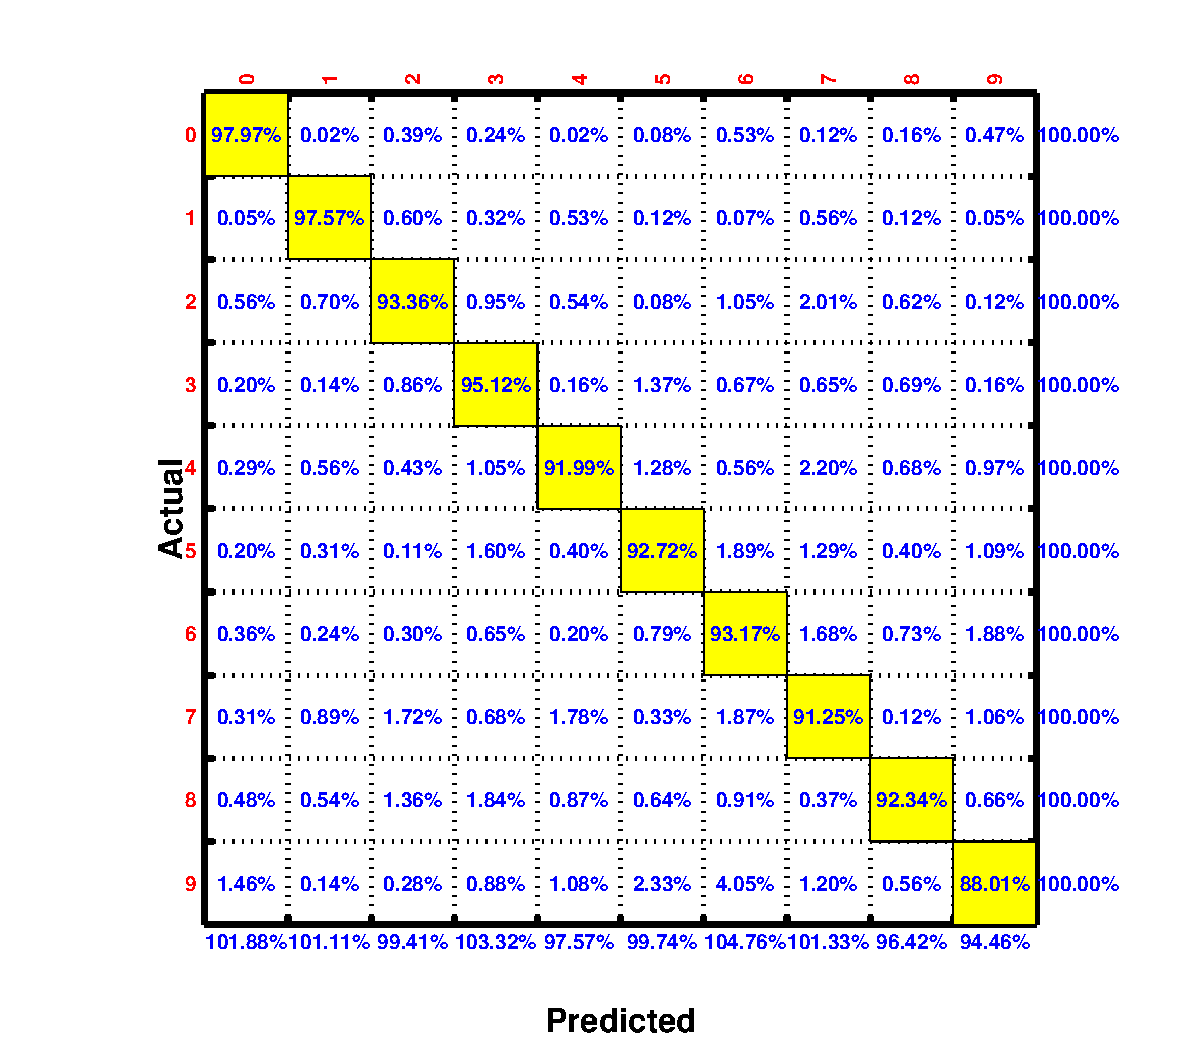
\includegraphics[width=0.5\textwidth]{confusionMat.eps}
\caption{\scriptsize Confusion matrix for the cNN classification. All training data was fed to the cNN. Each column of the matrix represents the percentages of instances in a predicted class, and each row represents the percentages of instances in an actual class. For example, the digit 9 has the lowest classification accuracy as it is often confused with the digit 6 due to the rotation applied.}
\label{confMat}
\end{figure}

\begin{figure}[H]
\centering
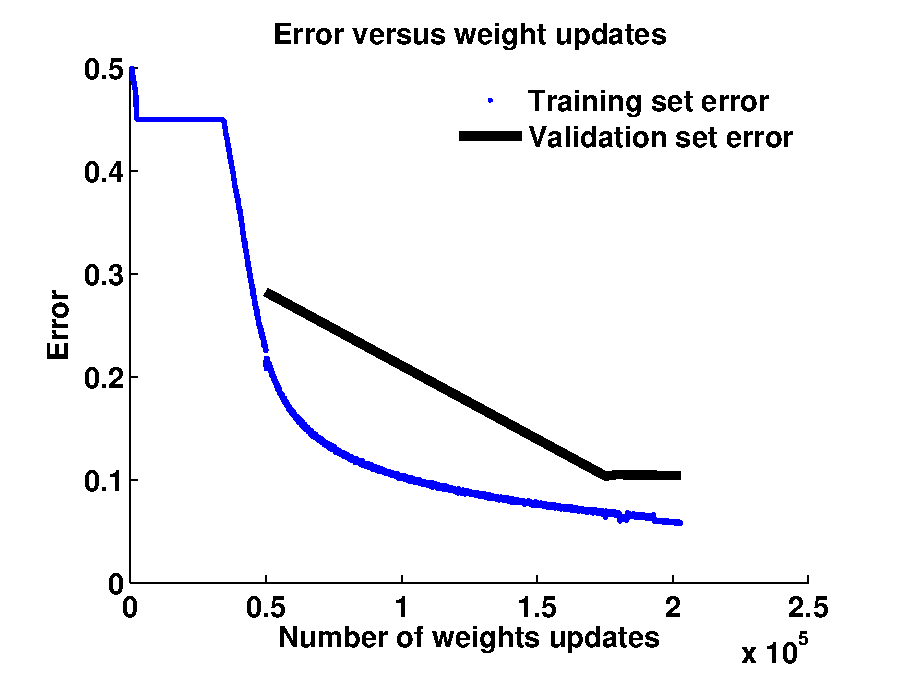
\includegraphics[width=0.5\textwidth]{erro.eps}
\caption{\scriptsize Training and validation error versus weight updates for the cNN. Mini-batches of 200 training examples were used. Therefore, there were $50,000/200=250$ weights updates in 1 epoch. Note that the validation set was only tested at limited number of iterations to save computation time with large-scale NN.}
\label{error}
\end{figure}

The cNN trains the filters in the convolution layers as feature extractors. The learned filters for images often resemble properties of neurons in the biological visual nervous system \cite{lecun-98}. The learned filters in each layer of the cNN are below.

\begin{figure}[H]
\centering
\includegraphics[width=0.4\textwidth]{feature1.png}
\caption{\scriptsize 6 filters of the 1st convolution layer.}
\label{feat1}
\end{figure}

\begin{figure}[H]
\centering
\includegraphics[width=0.4\textwidth]{feature2.png}
\caption{\scriptsize 16 filters of the 2nd convolution layer.}
\label{feat2}
\end{figure}

\begin{figure}[H]
\centering
\includegraphics[width=0.5\textwidth]{feature3.png}
\caption{\scriptsize 120 filters of the 3rd convolution layer.}
\label{feat3}
\end{figure}

\section{Discussion}
\subsection{Preprocessing and feature extraction for images of digits}
Aside from the cNN extracted features that will be discussed below (Figs. \ref{feat1}, \ref{feat2}, and \ref{feat3}), we found the PCA dimensionality reduction did not aid in improving the classification accuracy for the linear logistic regression classifier (Fig. \ref{lr}). In our attempt to find the pertinent features for the images of digits that might be useful in our case (Fig. \ref{ilastik} and \ref{rotate}). The only algorithm that benefited from the preprocessing was the feedforward NN. This could be due to that the hidden layers of the NN can theoretically approximate any nonlinear functions \cite{Min69, grossberg1973ces}, and this might enhance the classifier accuracy. Providing further support for this point, the linear Logistic Regression classifier and the linear SVM both performed worse with the preprocessing.

\subsection{Logistic regression, feedforward NN, and SVM}
We implemented these required algorithms for the report, however, we were surprised to find that they performed equally poorly in this classification task despite our attempt to optimize the preprocessing and feature extraction methods (Fig. \ref{compar}). In some cases, this was counter-intuitive, since the preprocessing that was able to bring out the prominent features to our eyes and brain only made the linear classifier perform worse (see results). This illustrates the high complexity of our visual nervous system to process images, and perhaps an algorithm inspired by the biological visual nervous system such as the cNN described below can offer insights into the problem of image classification \cite{lecun-98}.

\subsection{cNN outperforming the other algorithms}
We found cNN to significantly outperform the other methods by 0.5000 on average. The convolution layers are feature extractors trained through supervised learning. Only the last layer is a perceptron layer that performs the classification. Due to its deep architecture, there are many weights that need to be train with gradient descent, and the training time can be long. However, with the use of GPU computing, this was not a major issue for the Caffe implementation  \cite{DBLP:journals/corr/Krizhevsky14,jia2014caffe}. The cNN training is supervised and relies on the amount of training data. In our case, the 50,000 training examples was sufficient, and we rarely observed overfitting with the architectures we used (Fig. \ref{error}).\\
Also due to its deep architecture, we found the biggest hindrance to using convolutional neural networks can be the number of hyper-parameters that need to be optimized through cross-validation (Table. \ref{compar} and \ref{comparCNN}). Surprisingly, we found that the classification accuracy is largely insensitive to both alterations in the number of feature maps in each layer and the kernel size (Table. \ref{compar} and \ref{comparCNN}) (Of course, the number of feature maps should increase with layer depth as the finer features in the images are sought out, and kernel size should decrease with depth as the feature maps become smaller). These results show that convolutional neural networks are able to automatically extract pertinent features from the images through a supervised manner, achieving excellent accuracy without human invented preprocessing. In our case with the difficult MNIST plus dataset (Fig. \ref{ilastik} and \ref{rotate}), the cNN features are insensitive to scaling, rotations, shift, as well as added noise to the images. 

\subsection{General discussion}
In this paper, we found that cNN achieves an accuracy of 0.9304 in this difficult MNIST-plus data set (Fig. \ref{ilastik} and \ref{rotate}). With the use of GPU computing and parallelization tricks specifically designed for the cNN, this can be achieved within hours using around 10,000 iterations \cite{DBLP:journals/corr/Krizhevsky14,bottou-tricks-2012}. This is a realistic timeline to approach image classification problems in our daily lives. For example, we can obtain hundreds of thousands of training examples from a database of hand-written cheques, forms, and/or letters, and train the cNN feature extractors within hours before applying them to our classification problems. Also, once the convolution layers of the cNN are trained, we can readily use the cNN with any future testing examples. The supervised training of optimal feature extractors and the quick application of cNN makes it a powerful tool for image classification in the future \cite{DBLP:journals/corr/abs-1206-4656}. Future research on both the empirical applications and the theoretical analysis of the cNN might be fruitful for the machine learning community \cite{journals/cacm/Domingos12}.


\section*{Appendix}

The code used in this report can be found at the link below. The logistic regression algorithm was implemented in Matlab. The feedforward neural network trained by backpropagation was implemented in Python. The SVM numerical algorithms were implemented using Matlab toolboxes. The cNN algorithm was implemented from code developed by R. B. Palm \cite{IMM2012-06284} in Matlab, and Yangqing Jia \cite{jia2014caffe} in Python. The data for the digit classification can be downloaded from the Kaggle website and the code can be found at the link below. Samples of the preprocessed images can also be found here:\\
{\scriptsize https://github.com/npow/mnist}

$\checkmark$ \textbf{We hereby state that all work presented in this report is that of the authors.}

\printbibliography[heading=bibintoc,title={Reference}]
%\begin{thebibliography}{1}

%\bibitem{lecun-98}
%H.~Kopka and P.~W. Daly, \emph{A Guide to \LaTeX}, 3rd~ed.\hskip 1em plus
%  0.5em minus 0.4em\relax Harlow, England: Addison-Wesley, 1999.
%\end{thebibliography}

\end{document}

